\documentclass[../../main.tex]{subfiles}
\graphicspath{{\subfix{../../image/}}} % 指定图片目录,后续可以直接使用图片文件名。

% 例如:
% \begin{figure}[H]
% \centering
% \includegraphics[scale=0.4]{图.png}
% \caption{}
% \label{figure:图}
% \end{figure}
% 注意:上述\label{}一定要放在\caption{}之后,否则引用图片序号会只会显示??.

\begin{document}

\section{环同态}

\begin{definition}[环同态]
设$(R, +, \cdot) ,(R', +', *) $都是环,$f : (R, +, \cdot) \to (R', +', *) $ 是一个映射,我们说 $f$ 是个\textbf{环同态},若
\begin{enumerate}[(i)]
\item $f(1) = 1' ,$

\item $f(a + b) = f(a) +' f(b) ,$$\forall a,b\in R$.

\item $f(ab) = f(a) * f(b) ,$$\forall a,b\in R$.
\end{enumerate}
\end{definition}
\begin{remark}
未来,在不引起歧义的情况下,我们会忽略两个环中加法与乘法的区别,都记作 $+$ 和 $\cdot$,称环同态是
\begin{align*}
f : (R, +, \cdot) \to (R', +, \cdot) .
\end{align*}
\end{remark}

\begin{proposition}\label{proposition:环同态的等价条件}
设$(R, +, \cdot) ,(R', +', *) $都是环,$f : (R, +, \cdot) \to (R', +', *) $ 是一个映射,则$f$是环同态等价于$f$既是加法的群同态,又是乘法的幺半群同态.进而,$f$对加法保持逆元和单位元.
\end{proposition}
\begin{proof}
根据环同态的定义可直接得到,$f$是环同态等价于$f$既是加法的群同态,又是乘法的幺半群同态..再由\refpro{proposition:群同态保持逆元和单位元}可知,$f$对加法保持逆元和单位元.
\end{proof}

\begin{definition}[环同态的核与像]
设$f : (R, +, \cdot) \to (R', +', *) $是一个环同态,则我们定义 $f$ 的\textbf{核}与\textbf{像},记作 $\ker(f)$ 与 $\mathrm{im}(f)$,分别为
\begin{gather*}
\ker(f) = \{x \in R : f(x) = 0'\} \subset R ,\\
\mathrm{im}(f) = \{y \in R' : \exists x \in R, y = f(x)\} = \{f(x) : x \in R\} \subset R'.
\end{gather*}
\end{definition}
\begin{remark}
注意核在大多数情况下不会是一个子环.
\end{remark}

\begin{figure}[H]
\centering
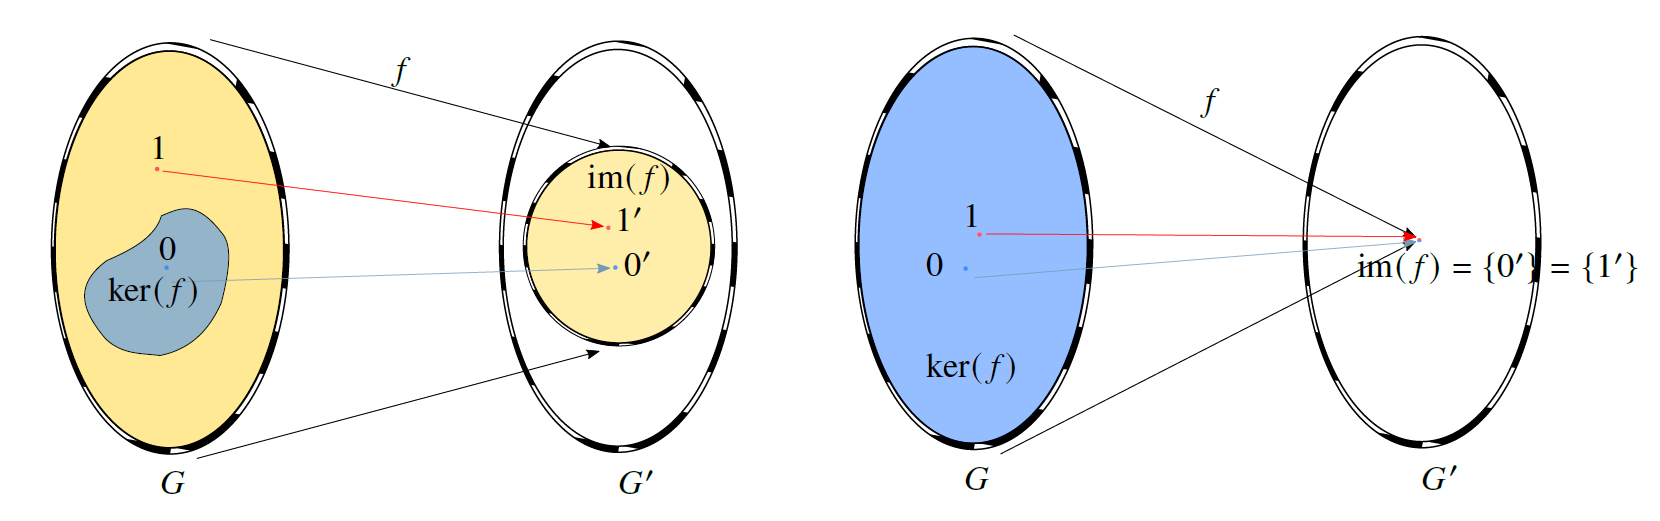
\includegraphics[scale=0.4]{环同态的核与像示意图.png}
\caption{环同态的核与像示意图}
\label{figure:环同态的核与像示意图}
\end{figure}

\begin{definition}[满同态与单同态]
设 $f:(R, +, \cdot) \to (R', +', *)$ 是一个环同态,我们称 $f$ 是一个\textbf{满同态}当 $f$ 是满射,称 $f$ 是一个\textbf{单同态}当 $f$ 是单射。 
\end{definition}

\begin{proposition}\label{proposition:一个环同态是单的当且仅当核是平凡的}
设  $f:(R, +, \cdot) \to (R', +', *)$ 是一个环同态,则
\begin{enumerate}
\item $f$ 是一个单同态当且仅当 $\ker(f)=\{0\}$。也就是说,一个环同态是单的当且仅当核是平凡的。

\item $f$ 是一个满同态当且仅当 $ \mathrm{im}(f)=R'$。也就是说,一个环同态是满的当且仅当值域等于陪域。
\end{enumerate}
\end{proposition}
\begin{proof}
证明与\refpro{proposition:一个环同态是单的当且仅当核是平凡的}类似.
\end{proof}


\begin{definition}[理想]
设 $(R, +, \cdot)$ 是一个环,而 $I \subset R$。我们定义,称 $I$ 是 $R$ 的\textbf{左理想},若
\begin{gather*}
(I, +) < (R, +),\\
\forall r \in R, \forall a \in I, ra \in I.
\end{gather*}
即$RI\subset I$,也即$RI=I.$也等价于$SI=I,\forall S\subset R$.

类似地,我们称 $I$ 是 $R$ 的\textbf{右理想},若
\begin{gather*}
(I, +) < (R, +),\\
\forall a \in I, \forall r \in R, ar \in I.
\end{gather*}
即$IR\subset I$,也即$IR=I.$也等价于$IS=I,\forall S\subset R$.

如果 $I$ 既是左理想又是右理想,我们就称 $I$ 是 $R$ 的一个\textbf{理想},记作 $I \lhd R$。 
\end{definition}
\begin{remark}
因为$(R,+)$是Abel群,所以$(I,+)是(R,+)$的子群等价于$(I,+)$是$(R,+)$的正规子群.
\end{remark}
\begin{note}
理想的第二条性质表明:理想在乘法下 “吸收” 了整个环到理想上,也就是说
\begin{align*}
RI \subset I\quad ,
IR \subset I.
\end{align*}
其中子集的乘法,定义为所有元素乘积的集合。而显然有$I\subset RI,IR$.故
\begin{gather*}
\forall r\in R,\forall a\in I,ra\in I\Leftrightarrow RI\subset I\Leftrightarrow RI=I,
\\
\forall r\in R,\forall a\in I,ar\in I\Leftrightarrow IR\subset I\Leftrightarrow IR=I.
\end{gather*}
\end{note}

\begin{lemma}\label{lemma:子环和理想与自身的乘积等于其自身}
\begin{enumerate}[(1)]
\item 设$(R,+,\cdot)$是一个环,$H< R$,则$HH=H$.

\item 设$(R,+,\cdot)$是一个环,$H\lhd R$,则$HH=H$.
\end{enumerate}
\end{lemma}
\begin{proof}
\begin{enumerate}[(1)]
\item 一方面,根据$H< R$可知, $H$是$R$的一个乘法子幺半群.于是由\reflem{lemma:子群或子幺半群与自身的乘积还等于其本身}可知,对 $\forall h_1,h_2\in H$,都有$h_1h_2\in H$。故 $HH\subset H$。

另一方面,设 $h\in H$,$e$是$R$的乘法单位元.则$h = he\in HH$。故 $H\subset HH$。

综上, $HH = H$。

\item 一方面,对 $\forall h_1,h_2\in H$,根据$H\lhd R$的定义及$h_1\in R$可知, $h_1h_2\in H$。故 $HH\subset H$。

另一方面,设 $h\in H$,$e$是$R$的乘法单位元.则$h = he\in HH$。故 $H\subset HH$。

综上,  $HH = H$。
\end{enumerate}
\end{proof}

\begin{lemma}[理想是整个环的充要条件]\label{lemma:理想是整个环的充要条件}
\begin{enumerate}[(1)]
\item 设 $(R, +, \cdot)$ 是一个环,而 $I \lhd R$。则 $I < R$ 当且仅当 $I = R$.

\item 设 $(R, +, \cdot)$ 是一个环,$1$ 是其乘法单位元,$I \lhd R$,则 $1 \in I$ 当且仅当 $I = R$。

\item 设 $(R, +, \cdot)$ 是一个环,$1$ 是其乘法单位元,$I \lhd R$,则 $R^{\times} \cap I \neq \varnothing$ 当且仅当 $I = R$。
\end{enumerate}
\end{lemma}
\begin{proof}
\begin{enumerate}[(1)]
\item 充分性是显然的,因为一个环当然是自己的子环.

我们来证明必要性。设 $I < R$,则特别地,$1 \in I$。可是 $I \lhd R$,因此对任何 $r \in R$,我们有
\begin{align*}
r = r \cdot 1 \in I.
\end{align*}
这就证明了 $I = R$。

综上所述,一个理想是子环当且仅当它是整个环.

\item 充分性是显然的。下证必要性。

由 $I \lhd R$ 可知 $I \subset R$。
因为 $1 \in I$,且 $I \lhd R$,所以 $\forall r \in R$,都有 $r = r \cdot 1 \in I$。因此 $R \subset I$。

综上,我们就有 $I = R$。

\item 充分性是显然的。下证必要性。

设 $a \in R^{\times} \cap I$,则 $a$ 是 $R$ 中的一个单位。从而存在 $b \in R$,使得 $ab = 1$。
又由 $I \lhd R$ 可知,$1 = ab \in I$。于是由 $(2)$ 可知 $I = R$。 
\end{enumerate}
\end{proof}

\begin{proposition}[理想的任意交还是理想]\label{proposition:理想的任意交还是理想}
设$(R,+,\cdot)$是一个环, $(N_i)_{i\in I}$ 是一族 $R$ 的理想,则它们的交集仍然是 $R$ 的理想,即
\begin{align*}
\bigcap_{i\in I}N_i\lhd R .
\end{align*}
\end{proposition}
\begin{proof}
一方面,
由条件可知,$((N_i)_{i\in I},+)$ 是一族 $(R,+)$ 的子群.从而由\refpro{proposition:子群的任意交仍是子群}可知$(\bigcap_{i\in I}N_i,+)$仍是$(R,+)$的子群.

另一方面,对$\forall r\in R$,$\forall n\in \bigcap_{i\in I}N_i$,都有$n\in N_i,\forall i\in I.$又因为对$\forall i\in I$,$N_i$都是$R$的理想,所以$rn\in N_i,\forall i\in I.$从而$rn\in \bigcap_{i\in I}N_i.$同理可证$nr\in \bigcap_{i\in I}N_i.$

综上,$\bigcap_{i\in I}N_i$仍然是 $R$ 的理想.
\end{proof}


\begin{proposition}\label{proposition:交换环的左理想、右理想、理想等价}
设 $(R, +, \cdot)$ 是一个交换环,则 $I$ 是一个左理想当且仅当 $I$ 是一个右理想,又当且仅当 $I$ 是一个理想。
\end{proposition}
\begin{proof}
根据交换环对乘法的交换律,这是显然的.
\end{proof}

\begin{proposition}\label{proposition:nZ是Z的理想}
设 $n \in \mathbb{N}_1$,则 $n\mathbb{Z}$ 是 $\mathbb{Z}$ 的理想,即
\begin{align*}
n\mathbb{Z} \lhd \mathbb{Z} .
\end{align*}
\end{proposition}
\begin{proof}
首先,由\refpro{proposition:nZ是Z的正规子群}我们知道 $(n\mathbb{Z}, +)$ 是 $(\mathbb{Z}, +)$ 的(加法)正规子群。

其次,注意到 $\mathbb{Z}$ 是一个交换环,故根据\refpro{proposition:交换环的左理想、右理想、理想等价}可知,我们只须证明 $n\mathbb{Z}$是$\mathbb{Z}$的左理想,也即 $\mathbb{Z} \cdot n\mathbb{Z} \subset n\mathbb{Z}$。

要证明 $\mathbb{Z} \cdot n\mathbb{Z} \subset n\mathbb{Z}$,我们只须令 $m \in \mathbb{Z}$, $nk \in n\mathbb{Z}(k \in \mathbb{Z})$,只要证明 $mnk \in n\mathbb{Z}$ 即可。而这是因为
\begin{align*}
mnk = n(mk) \in n\mathbb{Z} .
\end{align*}
综上所述,这就证明了 $n\mathbb{Z}$ 是 $\mathbb{Z}$ 的理想。 
\end{proof}

\begin{lemma}
设 $n \in \mathbb{N}_1$,我们要定义映射 $f : (\mathbb{Z}, +, \cdot) \to (\mathbb{Z}_n, +, \cdot)$。对 $m \in \mathbb{Z}$,我们定义
\begin{align*}
f(m) = m + n\mathbb{Z} .
\end{align*}
则 $f$ 是一个环同态,而 $\ker(f) = n\mathbb{Z} \lhd R$。
\end{lemma}
\begin{proof}
先证明 $f$ 是加法的群同态。

设 $a, b \in \mathbb{Z}$,由\refpro{proposition:nZ是Z的正规子群}可知,$(n\mathbb{Z},+)\lhd(\mathbb{Z},+)$.从而
\begin{align*}
f(a)+f(b)=a+n\mathbb{Z}+b+n\mathbb{Z} = a+b+n\mathbb{Z}=f(a+b).
\end{align*}
故$f$ 是加法的群同态。

下面证明 $f$ 是乘法的幺半群同态。

第一,$f(1) = 1 + n\mathbb{Z}$ 是 $\mathbb{Z}_n$ 的乘法单位元。

第二,设 $m, m' \in \mathbb{Z}$,则利用上一章中我们证明过的 $\mathbb{Z}_n$ 对乘法的良定义性,我们有
\begin{align*}
f(m)f(m') = (m + n\mathbb{Z})(m' + n\mathbb{Z}) = mm' + n\mathbb{Z} = f(mm') .
\end{align*}
故$f$ 是乘法的幺半群同态。

综上所述,$f$ 是一个从 $\mathbb{Z}$ 到 $\mathbb{Z}_n$ 的环同态。 

注意到
\begin{align*}
\mathrm{ker}f=\{m\in \mathbb{Z} :f(m)=n\mathbb{Z} =\overline{0}\}=\{m\in \mathbb{Z} :\overline{m}=m+n\mathbb{Z} =n\mathbb{Z} =\overline{0}\}=\{m\in \mathbb{Z} :m\in n\mathbb{Z} \}=n\mathbb{Z} .
\end{align*}
因此由\refpro{proposition:nZ是Z的理想}可知$\ker(f) = n\mathbb{Z} \lhd R$。
\end{proof}

\begin{proposition}[环同态的核是理想并且像是子环]\label{proposition:环同态的核是理想并且像是子环}
设 $f : (R, +, \cdot) \to (R', +, \cdot)$ 是一个环同态,则 $f$ 的核是 $R$ 的理想,$f$ 的像是 $R'$ 的子环。此即,
\begin{gather*}
\ker(f) = \{a \in R : f(a) = 0'\} \lhd R,\\
\mathrm{im}(f) = \{b \in R' : \exists a \in R, b = f(a)\} = \{f(a) \in R' : a \in R\} < R'.
\end{gather*}
\end{proposition}
\begin{proof}
我们先证明 $\ker(f) \lhd R$。根据群同态的性质,由\hyperref[theorem:群同构第一定理]{群同构第一定理},我们知道 $\ker(f)$ 是加法的(正规)子群。为了方便起见,令 $I = \ker(f)$。我们只须证明 $RI \subset I$ 以及 $IR \subset I$。

令 $a \in R$,$b \in I = \ker(f)$,故 $f(b) = 0'$。因此,$f(ab) = f(a)f(b) = f(a)0' = 0'$,从而 $ab \in \ker(f) = I$。这就证明了 $RI \subset I$。而另一个包含关系同理可证。这样,我们就证明了 $\ker(f) \lhd R$。

我们再证明 $\mathrm{im}(f) < R'$。第一,$1' = f(1) \in \mathrm{im}(f)$。

第二,令 $a', b' \in \mathrm{im}(f)$,不妨设 $a' = f(a)$,$b' = f(b)$。只须证明 $a' - b', a'b' \in \mathrm{im}(f)$。而由$f$对加法是群同态可知,$f$保持加法逆元和加法.由$f$对乘法是幺半群同态可知,$f$保持乘法.于是就有
\begin{align*}
a' - b' &= f(a) - f(b) = f(a - b) \in \mathrm{im}(f) ,\\
a'b' &= f(a)f(b) = f(ab) \in \mathrm{im}(f)。
\end{align*}

这就证明了 $\mathrm{im}(f) < R'$。

综上所述,我们证明了这个命题。 
\end{proof}

\begin{definition}[商环]\label{definition:商环}
设 $(R, +, \cdot)$ 是一个环,而 $I \lhd R$。我们定义 $R$ 对 $I$ 的\textbf{商环},定义为 $(R/I, +, \cdot)$,其中
\begin{align*}
R/I = \{a + I : a \in R\}.
\end{align*}
而加法和乘法分别对 $a + I, b + I \in R/I (a, b \in R)$,定义为
\begin{align*}
(a + I) + (b + I) &= (a + b) + I,\\
(a + I)(b + I) &= (ab) + I.
\end{align*} 
\end{definition}
\begin{proof}
我们需要证明上述定义是良定义的,即证上述的加法和乘法是良定义的,且商环$(R,+,\cdot)$是一个环.

注意到$(R,+)$是Abel群,又因为$I$是$R$的理想,所以$(I,+)$是$(R,+)$的子群.从而由\refpro{proposition:阿贝尔群的子群与正规子群等价}可知$(I,+)$是$(R,+)$的正规子群.根据\refpro{proposition:陪集乘法的良定义性}可知,正规子群$I$的陪集的加法是良定义的,即上述加法是良定义的.

我们要证明商环对乘法是良定义的。令 $a + I = a' + I$,$b + I = b' + I$,即 $a - a' \in I$,$b - b' \in I$。我们只须证明 $ab + I = a'b' + I$,即 $ab - a'b' \in I$。而这是因为
\begin{align*}
ab - a'b' &= (ab - a'b) + (a'b - a'b') = (a - a')b + a'(b - b') \in IR + RI \subset I + I = I .
\end{align*}
其中倒数第二个包含关系是根据理想对乘法的 “吸引” 性质,而最后一个等号是根据\reflem{lemma:子群或子幺半群与自身的乘积还等于其本身}及$(I,+)<(R,+)$。这样,我们就证明了商环对乘法是良定义的。

接下来,要证明商环是个环,其实只要将 $R$ 上环的结构(利用良定义性)照搬过来即可。

利用 $I$ 对加法构成正规子群,因此利用\refpro{proposition:商群}可知,$R/I$ 对加法构成群。我们只须证明 $R/I$ 对乘法构成幺半群,且乘法对加法有左右分配律。

乘法单位元是 $1 + I$,因为对任意 $a + I (a \in R)$,我们有
\begin{align*}
(a + I)(1 + I) = (1 + I)(a + I) = a + I 。
\end{align*}

$R/I$ 对乘法有结合律,这是因为对任意 $a + I, b + I, c + I (a, b, c \in R)$,由$(R,+,\cdot)$是一个环可得
\begin{align*}
((a + I)(b + I))(c + I) = (ab + I)(c + I) = (ab)c + I = a(bc) + I = (a + I)((b + I)(c + I)) 。
\end{align*}
最后,我们要证明乘法对加法有左右分配律。利用对称性,我们只证明左分配律。对任意 $a + I, b + I, c + I (a, b, c \in R)$,由$(R,+,\cdot)$是一个环可得
\begin{align*}
(a + I)((b + I) + (c + I)) &= (a + I)((b + c) + I) = a(b + c) + I \\
&= (ab + ac) + I = (a + I)(b + I) + (a + I)(c + I).
\end{align*}

综上所述,我们就证明了 $R/I$ 是个环。这个环被叫做 $R$ 对 $I$ 的商环。 
\end{proof}

\begin{definition}[环同构]
设 $(R, +, \cdot),(R', +, \cdot)$ 都是环,$f : (R, +, \cdot) \to (R', +, \cdot)$ 是一个映射,我们称 $f$ 是一个\textbf{环同构},若 $f$ 既是双射,又是环同态。
\end{definition}

\begin{lemma}\label{lemma:环同构等价于对加法是群同构对乘法是幺半群同构}
设 $(R, +, \cdot),(R', +, \cdot)$ 都是环,$f : (R, +, \cdot) \to (R', +, \cdot)$ 是一个映射,则$f$ 是环同构,当且仅当 $f$ 对加法是群同构,而对乘法是幺半群同构。
\end{lemma}
\begin{proof}
必要性是显然的.下证充分性.

由于$f$ 对加法是群同构,而对乘法是幺半群同构,因此$f$是双射,且$f$既对加法是群同态,又对乘法是幺半群同态.于是由\refpro{proposition:环同态的等价条件}可知$f$是环同态.又因为$f$是双射,所以$f$是环同构.
\end{proof}

\begin{lemma}\label{lemma:环同构的逆还是环同构}
设 $(R, +, \cdot),(R', +, \cdot)$ 都是环, $f : (R, +, \cdot) \to (R', +, \cdot)$ 是个环同构,则 $f^{-1}$ 是个环同态,进而也是环同构。
\end{lemma}
\begin{proof}
由$f$是个环同构可知,$f$既对加法是群同态,又对乘法是幺半群同态..从而由\refpro{proposition:幺半群同构的逆是幺半群同态}和\refpro{proposition:群同构的逆也是群同构}可知, $f^{-1}$ 既对加法是群同态,又对乘法是幺半群同态.于是由\refpro{proposition:环同态的等价条件}可知$f$是环同态.又因为$f^{-1}$是双射,所以$f^{-1}$是环同构.
\end{proof}

\begin{theorem}[环同构第一定理]\label{theorem:环同构第一定理}
设$f : (R, +, \cdot) \to (R', +, \cdot)$ 是一个环同态,则 $R$ 对 $\ker(f)$ 构成的商环,同构于 $\mathrm{im}(f)$。此即,
\begin{align*}
R / \ker(f) \cong \mathrm{im}(f) .
\end{align*}
\end{theorem}
\begin{proof}
令 $\tilde{f} : R / \ker(f) \to \mathrm{im}(f)$,对 $a + \ker(f)$,定义为
\begin{align*}
\tilde{f}(a + \ker(f)) = f(a) .
\end{align*}
我们根据\hyperref[theorem:群同构第一定理]{群同构第一定理中对$\tilde{f}$的证明}同理可证 $\tilde{f}$ 是良定义的,且对加法构成群同构.要证明 $\tilde{f}$ 是环同构,只须证明它对乘法是幺半群同态。

单位元:由\hyperref[definition:商环]{商环的定义}及\refpro{proposition:环同态的核是理想并且像是子环}可知,$R / \ker(f)$的乘法单位元是$1+\ker f$且$\mathrm{im}(f)<R'$,从而$\mathrm{im}(f)$的乘法单位元就是$R'$的乘法单位元.由$\tilde{f}$的定义及$f$是环同态可得$\tilde{f}(1+\ker f)=f(1)=1'.$

保持乘法:令 $a + \ker(f), b + \ker(f) \in R / \ker(f) (a, b \in R)$,则
\begin{align*}
\tilde{f}((a + \ker(f))(b + \ker(f))) = \tilde{f}(ab + \ker(f)) = f(ab) = f(a)f(b) = \tilde{f}(a + \ker(f))\tilde{f}(b + \ker(f)).
\end{align*}
综上所述,$\tilde{f}$ 给出了一个从商环 $R / \ker(f)$ 到像 $\mathrm{im}(f)$ 的环同构。这就证明了这个定理。
\end{proof}

\begin{theorem}[环同构第二定理]\label{theorem:环同构第二定理}
设$(R, +, \cdot)$ 是一个环,而 $S < R$,$I \lhd R$。则 $S + I < R$,$S \cap I \lhd S$,$I \lhd S + I$,且
\begin{align*}
S / (S \cap I) \cong (S + I) / I.
\end{align*}
\end{theorem}
\begin{proof}
我们先证明 $S + I < R$。对加法而言,由$S<R,I\lhd R$可知$(S,+)< (R,+),(I,+)<(R,+)$,又因为$(R,+)$是Abel群,所以$(S,+),(I,+)\lhd (R,+)$.
从而由\reflem{lemma:HN<G的条件}可知$(S+I,+)<(R,+)$.因此我们只须证明 $S + I$ 对乘法构成幺半群,即对乘法是封闭的,且包含单位元。第一,$1 = 1 + 0 \in S + I$。第二,只须证明 $(S + I)(S + I) \subset (S + I)$.由\reflem{lemma:子环和理想与自身的乘积等于其自身}可知$II=I$,由\reflem{lemma:子群或子幺半群与自身的乘积还等于其本身}可知$SS=S,I+I=I$.根据$I\lhd R$可知$IS,SI= I.$于是再利用$R$的乘法对加法满足左右分配律可得
\begin{align*}
(S + I)(S + I) = SS + SI + IS + II = S + I + I + I = S + I .
\end{align*}

我们再证明 $S \cap I \lhd S$。由\refpro{proposition:子群的任意交仍是子群}可知,$S \cap I$ 对加法构成子群。我们只须证明 $S \cap I$ 对乘法的 “吸收” 性,即 $(S \cap I)S \subset S \cap I$,及 $S(S \cap I) \subset S \cap I$。根据对称性,我们只证明前面这个包含关系。由$SS=S,IS=I$可得
\begin{align*}
(S\cap I)S\subset SS=S,(S\cap I)S\subset IS=I
\Leftrightarrow
(S \cap I)S = S \cap IS = S \cap I .
\end{align*}
根据对称性,$S \cap I \lhd S$。

我们接着证明 $I \lhd S + I$.我们已经证明了$S+I<R$,因此$S+I$对加法构成Abel群,又$I\subset S+I$($0\in S,I=0+I\subset S+I$),故$(I,+)<(S+I,+)$.于是我们只须证明 $I(S + I) \subset I$,及 $(S + I)I \subset I$。根据对称性,我们只证明前面这个包含关系。由$I\lhd R$及$S+I\subset R$可得
\begin{align*}
I(S + I) = IS + II = I + I = I.
\end{align*}
根据对称性,$I \lhd S + I$。

我们最后证明 $S / (S \cap I) \cong (S + I) / I$。和\hyperref[theorem:群同构第二定理]{群同构第二定理的证明}一样,我们定义 $f : S \to (S + I) / I$,对 $a \in S$,定义为
\begin{align*}
f(a) = a + I \in (S + I) / I.
\end{align*}
先证$f$ 是良定义的.设$a=a'\in S,$则$a-a'=0\in I$,从而$f(a)=a+I=a'+I=f(a')$.故$f$是良定义的.
显然$f$是满射,又由\hyperref[theorem:群同构第二定理]{群同构第二定理的证明}可知,$f$对加法构成群同态,且 $\mathrm{ker(}f)=\left\{ a\in S:a+I=I \right\} =\left\{ a\in S:a\in I \right\} =S\cap I.$因此我们只要证明 $f$ 对乘法是幺半群同态,就可以利用\hyperref[theorem:环同构第一定理]{环同构第一定理}证明这个命题了。而这是显然的,因为若 $a, b \in S$,则
\begin{align*}
f(a)f(b) = (a + I)(b + I) = ab + I = f(ab).
\end{align*}
因此,由\hyperref[theorem:环同构第一定理]{环同构第一定理},我们得到了
\begin{align*}
S / (S \cap I) \cong (S + I) / I .
\end{align*}

综上所述,我们就证明了这个命题。
\end{proof}

\begin{lemma}\label{lemma:理想的"传递性"}
设$(R,+,\cdot)$是一个环,$I\lhd R,J<R$,且$I\subset J$,则$I\lhd J$.
\end{lemma}
\begin{proof}
第一,由 $I \lhd  R$ 可知 $(I, +) < (R, +)$,从而 $I$ 对单位、加法和逆元都封闭。又 $I \subset J$,故 $(I, +) < (J, +)$。

第二,由 $J < R$ 可知 $J \subset R$。于是由 $I \lhd  R$ 可得 $IJ = JI = I$。

综上,$I \lhd  J$。 
\end{proof}

\begin{theorem}[环同构第三定理]\label{theorem:环同构第三定理}
设 $(R, +, \cdot)$ 是一个环,而 $I, J \lhd R$,且 $I \subset J$。则 $J / I \lhd R / I$,且
\begin{align*}
(R / I) / (J / I) \cong R / J 。
\end{align*}
\end{theorem}
\begin{proof}
首先,由\reflem{lemma:理想的"传递性"}可知$I\lhd J$.故$J / I$是一个商环.由 $I, J \lhd R$可知$R/I,R/J$也是商环.
我们先证明 $J / I \lhd R / I$。对加法而言$J / I$ 和 $R / I$都是群,从而它们都对单位元、加法和逆元封闭.又$J / I\subset R / I$,故 $J / I$ 是 $R / I$ 的加法子群。我们只须证明 $(J / I)(R / I) \subset J / I$,及 $(R / I)(J / I) \subset J / I$。根据对称性,我们证明前面这个包含关系。因为 $J \lhd R$,所以
\begin{align*}
(J / I)(R / I) = (JR) / I \subset J / I .
\end{align*}
这就证明了 $J / I \lhd R / I$。

和\hyperref[theorem:群同构第三定理]{群同构第三定理}一样,我们令 $f : R / I \to R / J$,对 $a + I (a \in R)$,定义为
\begin{align*}
f(a + I) = a + J .
\end{align*}

根据\hyperref[theorem:群同构第三定理]{群同构第三定理的证明},同理可知$f$ 是一个良定义的满射,对加法构成群同态,且 $\ker(f) = J / I$。因此我们只要证明 $f$ 对乘法是幺半群同态,就可以利用环同构第一定理证明这个命题了。而这是显然的,因为若 $a + I, b + I \in R / I (a, b \in R)$,则
\begin{align*}
f(a + I)f(b + I) = (a + J)(b + J) = ab + J = f(ab + I).
\end{align*}
又因为$f(1+I)=1+J$.
因此,由\hyperref[theorem:环同构第一定理]{环同构第一定理},我们得到了
\begin{align}
(R / I) / (J / I) \cong R / J.
\end{align}

综上所述,我们就证明了这个命题。 
\end{proof}









\end{document}